\section{Concrete arithmetic and algebraic examples}\label{sec:applications}

\subsection{A three-character entire function}

For clarity, an explicit instance uses the three primitive real characters
\[
 \chi_3=(0,1,-1),\quad
 \chi_4=(0,1,0,-1),\quad
 \chi_5=(0,1,-1,-1,1),
\]
listed in residue order from zero.  The first two are odd and the third is
even.  Write $a_3=a_4=1$ and $a_5=0$, and define
\[
 F_q(z)=
 \left(\frac q\pi\right)^{(1/2+iz+a_q)/2}
 \Gamma\!\left(\frac{1/2+iz+a_q}{2}\right)
 L(1/2+iz,\chi_q),\qquad q\in\{3,4,5\}.
\]
Their Gauss sums are respectively $i\sqrt3$, $2i$, and $\sqrt5$;
dividing by $i^{a_q}\sqrt q$ gives root number $1$.
Thus their completed functional equations show that they are
real entire and even in $z$.  Their zeros are real by Dirichlet GRH.
The entire meaning includes the removable singularities at the gamma
factor's poles.\cite{dlmfdirichlet}

Place $F_3,F_4,F_5$ on a path in that order, with positive conductances
$a,b$.  The forest sum is the following explicit entire function:
\begin{align}\label{eq:three-character}
 \mathcal H_{a,b}(z)={}&F_3'F_4'F_5'
  +aF_3F_4'F_5'+(a+b)F_3'F_4F_5'
  +bF_3'F_4'F_5 \notag\\
 &+ab(F_3F_4F_5)'.
\end{align}
Every factor in this display is evaluated at $z$.
The entire-function theorem proves that \emph{every zero of
$\mathcal H_{a,b}$ is real}, for every $a,b>0$.
Equivalently, all zeros of
$\mathcal H_{a,b}(-i(s-1/2))$ lie on $\Re s=1/2$.

This example has an exactly known central zero.  For $s>0$, the block sums
for $L(s,\chi_3)$ and $L(s,\chi_4)$ are strictly positive.  For $\chi_5$
the block is
\[
 (5k+1)^{-s}-(5k+2)^{-s}-(5k+3)^{-s}+(5k+4)^{-s}>0,
\]
because $x^{-s}-(x+1)^{-s}$ is strictly decreasing in $x>0$.
These grouped series converge and agree with the analytic continuation
in $\Re s>0$ by Dirichlet's test.  Hence $F_q(0)>0$ for all three
characters.  Since each $F_q$ is even, $F_q'(0)=0$.  The complementary
matrix at zero is the connected path Laplacian and has nullity one.
The exact multiplicity theorem therefore shows that zero is a
\emph{simple} zero of $\mathcal H_{a,b}$.

There is also a direct check.  With $m_q=F_q'/F_q$, each $m_q'(0)<0$.
The terms in \eqref{eq:three-character} involving at least two derivatives
vanish to order at least two.  Therefore
\[
 \mathcal H_{a,b}'(0)=ab\,F_3(0)F_4(0)F_5(0)
                       \sum_{q=3,4,5}m_q'(0)<0.
\]
No simplicity or distinctness assumption about any noncentral Dirichlet
zeros is used.

\subsection{Finite packets of arithmetic zeros}

For each of finitely many primitive characters, select any nonempty finite
multiset of zero ordinates of its phase-real completion, preserving the
selected multiplicities.  Form the monic polynomial whose roots are those
ordinates.  Theorem~\ref{thm:electrical} applies immediately: the exact
average shift from the critical points of their product is given by the
effective resistances and the numbers of chosen zeros.  The same
electrical answer holds for a completely different selection with the
same cardinalities.  Thus the formula makes a statement about actual
Dirichlet zero packets while requiring no knowledge of their numerical
locations to compute the displacement budget.

This assertion concerns finite packets.  It does not claim that unnormalized
truncated polynomial graph sums converge to the entire graph sum, nor
that the finite displacement sum can be passed to an infinite sum.
Canonical products have exponential normalization factors; the direct
entire-function proof accounts for them instead.

\subsection{Three quadratics and a zero collision}

Take $p_1=z^2-1$, $p_2=z^2-4$, $p_3=z^2-9$ on the path with common
conductance $t$.  Exact expansion gives
\begin{align*}
 \mathcal P_t(z)
 =2z\bigl(3t^2z^4+8tz^3+(4-28t^2)z^2-36tz+49t^2\bigr).
\end{align*}
The critical points of $p_1p_2p_3$ are
\[
 -\sqrt7,\quad-\sqrt{7/3},\quad0,\quad\sqrt{7/3},\quad\sqrt7.
\]
Their mean ordered displacement from the five graph zeros is exactly
$8/(15t)$.  Figure~\ref{fig:quadratics} shows the monotone motion.

At $t=1$ the graph polynomial factors as
\[
 \mathcal P_1(z)=2z(z-1)(3z^3+11z^2-13z-49).
\]
Its zeros are approximately
\[
 -3.6158196613,\quad-2.1509430367,\quad0,\quad1,\quad2.1000960313.
\]
The zero at $1$ coincides with an input root.  At that point the
complementary matrix on vertices $2,3$ is
\[
 \begin{pmatrix}4/3&-1\\-1&3/4\end{pmatrix},
\]
which has nullity one.  The multiplicity formula correctly gives one
output zero there, although the input root itself is simple.  This is a
useful case for testing cancellation of the apparent logarithmic poles.

Add an edge of conductance $h$ between vertices $1$ and $3$.
For the original path $R_{13}=2$, $L^+(e_1-e_3)=(1,0,-1)^{\mathsf T}$,
and $\|q_{13}\|^2=4$.  The total motion of the five ordered graph zeros is
therefore
\[
 \sum_{k=1}^5\bigl(\lambda_k(G_h)-\lambda_k(G)\bigr)
 =\frac{4h}{1+2h}.
\]
At $h=1$ it is exactly $4/3$.  The derivative of the new complementary
determinant at the former collision is not needed: that determinant is
already $4h/3$, so the root ceases to coincide with the input root for
every $h>0$.

\begin{figure}[tbp]
 \centering
 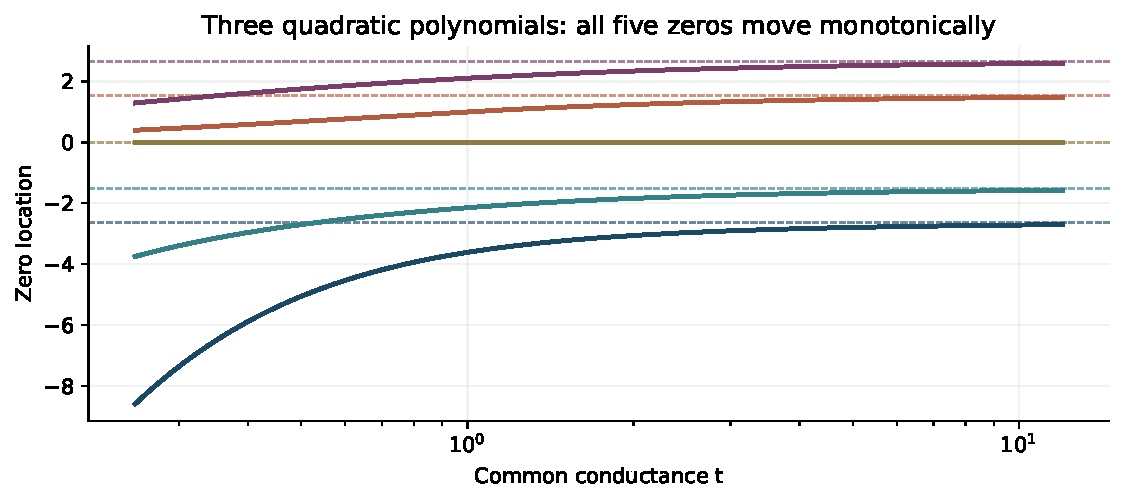
\includegraphics[width=.92\textwidth]{figures/quadratic_flow.pdf}
 \caption{The five graph zeros for three quadratic inputs.
 Dashed lines are the critical points of the input product.
 The zero at zero is fixed; all ordered curves are nondecreasing.
 The exact mean gap is $8/(15t)$.}
 \label{fig:quadratics}
\end{figure}

\subsection{A stronger collision used in verification}

The exact checker also uses $p_1=z^2$, $p_2=z(z-2)$, $p_3=(z-1)(z-3)$,
with path conductances $1$ and $4/3$.  It obtains
\[
 \mathcal P_G(z)=\tfrac43z^2(6z^3-16z^2-7z+26).
\]
At zero the input multiplicities are $2,1,0$.  The forced contribution
is $(2-1)+(1-1)=1$, while the one-dimensional complementary matrix
vanishes, adding one more zero.  Increasing the second conductance to
$5/3$ removes this extra nullity; the order at zero becomes one.  The
total movement of all ordered zeros is exactly $1/5$.
